\documentclass[10pt,conference,compsocconf]{IEEEtran}

\usepackage[colorlinks,allcolors=blue]{hyperref}  % Clickable links
\usepackage{xurl}
\usepackage{graphicx}	% For figure environment
\usepackage{csquotes}
\usepackage[english]{babel}
% \usepackage[inline]{enumitem} % Consider uncommenting if needed for specific lists later


\usepackage[
    backend=biber,      % Use biber backend for modern bibliography processing
    style=ieee,         % IEEE citation style
    citestyle=numeric-comp, % Compressed numeric citations [1-3] instead of [1,2,3]
    natbib=true,        % Enable natbib compatibility commands
    % Advanced options (uncomment as needed):
    maxnames=3,     % Maximum number of author names to display
    % minnames=1,       % Minimum number of author names before "et al."
    % doi=false,        % Disable DOI display in bibliography
    isbn=false,       % Disable ISBN display in bibliography
    url=false,        % Disable URL display in bibliography
    date=year,        % Show only year in dates
    % giveninits=false, % Show full author first names
]{biblatex}
\addbibresource{literature.bib}  % Your bibliography database
\DefineBibliographyStrings{english}{andothers = {et al\adddot}}
\AtEveryBibitem{\clearfield{pages}} % Remove page numbers from bibliography entries

\begin{document}
\title{HappiScope: Exploring the Multidimensional Nature of Global Happiness}

\author{%
  \makebox[\textwidth][c]{% center the box
    \begin{minipage}{1.5\textwidth} % Adjusted width slightly if needed for alignment
    \vspace{-1em}%
      \centering%
  Chang Jin	(403930),
Rizhong Lin	(366842),
Anlan Wang	(403909)\\
  \textit{COM-480 Data Visualization -- Milestone 2}
      \vspace{-1em}%
    \end{minipage}%
  }%
}

\maketitle

% ---------- Project Vision ----------
\section{Project Vision and Current Status}
The HappiScope project aims to develop an interactive web-based platform for visualizing the World Happiness Report data from 2015 to 2024. Our goal is to provide an intuitive interface for users—including policymakers, researchers, educators, and the general public—to explore global happiness trends, understand the contributing factors (such as social support, healthy life expectancy, freedom, generosity, and corruption perception), and analyze correlations with other key indicators like population and the Human Development Index (HDI). The platform seeks to facilitate the discovery of geographic disparities, temporal patterns, and complex socioeconomic relationships related to well-being.

A preliminary version of the HappiScope website, showcasing the planned structure and basic components, is currently accessible at: \url{https://com-480-data-visualization.github.io/HappiScope/}.

% ---------- Core Visualization Components ----------
\section{Core Visualization Components}
The final HappiScope platform will feature four primary interactive visualization components, as conceptualized in Figure~\ref{fig:sketches}. These components are designed to offer distinct perspectives for exploring and interpreting the multifaceted happiness data.

\begin{figure*}[ht]
    \centering
    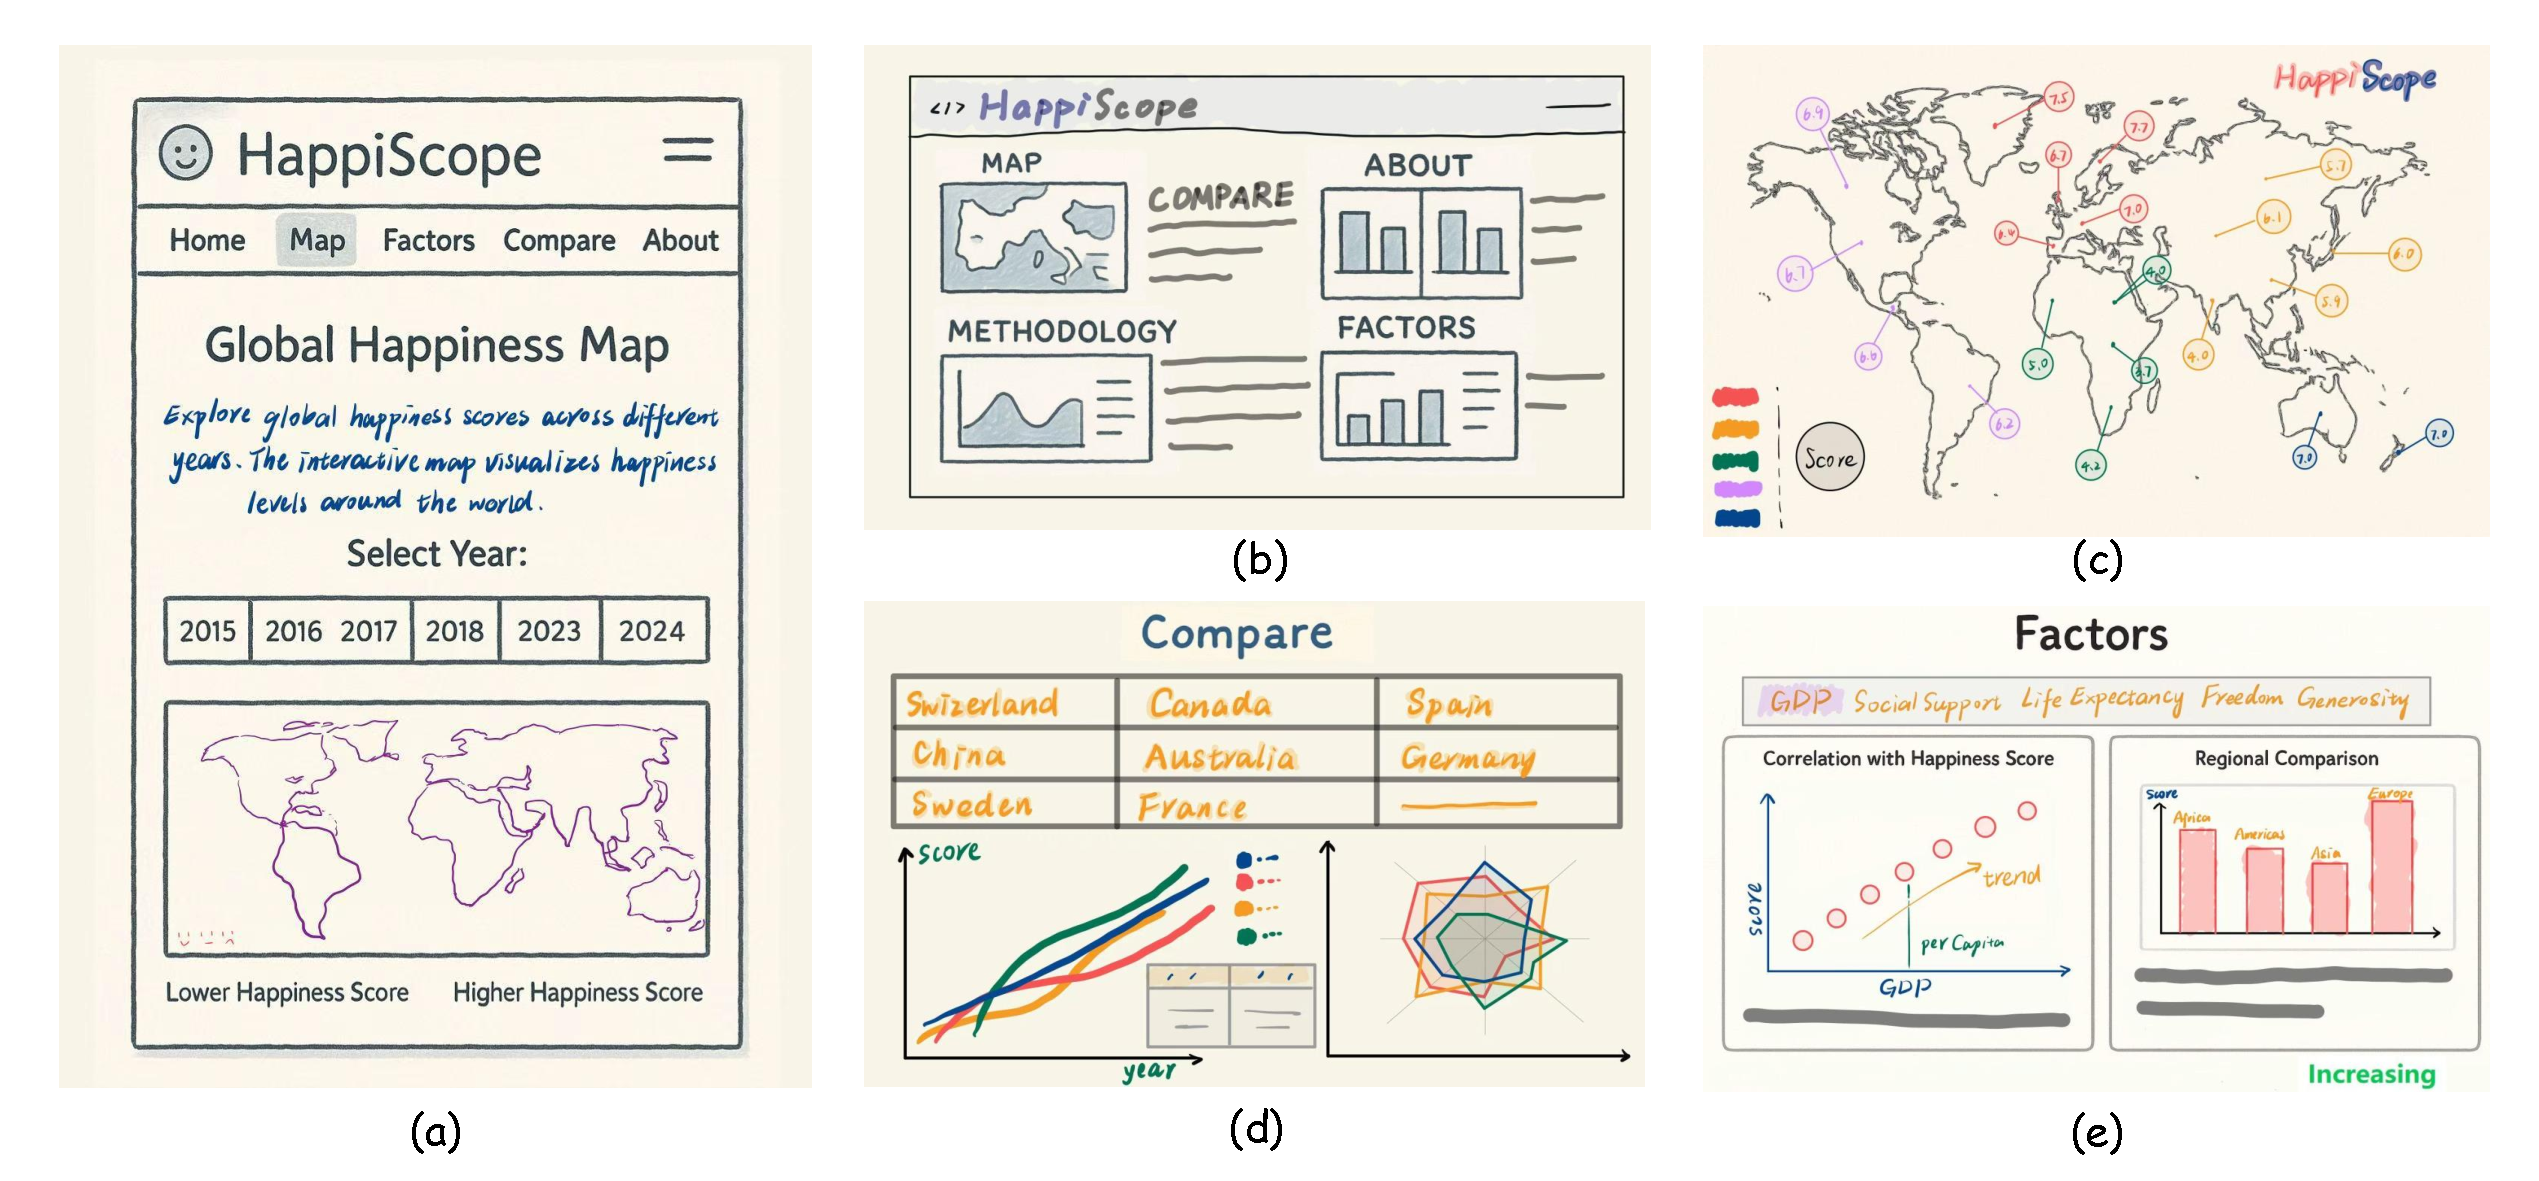
\includegraphics[width=\linewidth]{sketches.pdf}
    \caption{Key visualization components planned for the HappiScope platform: (a) Geographic visualization interface featuring timeline controls for temporal exploration; (b) Main dashboard providing an overview and access to different visualization modules; (c) Interactive world map displaying happiness scores or other selected metrics, with country-level details available on hover; (d) Country comparison view enabling multi-variable analysis between selected nations; and (e) Correlation analysis interface designed for exploring relationships between happiness factors and other indicators.}
    \label{fig:sketches}
\end{figure*}

\subsection{Overall Interface Dashboard}
\subsubsection{Description}
A well-organized landing page will serve as the central hub, presenting an overview panel of the available visualizations as shown in Figure~\ref{fig:sketches}(b). This includes thumbnail previews of each visualization module (Map, Comparison, Factor Analysis, etc.), allowing users to quickly browse and select the ones they wish to explore in detail.
\subsubsection{Goal}
Provide users with an intuitive entry point to explore the data from different analytical perspectives.
\subsubsection{Tools}
The interface will be built using standard web technologies: HTML, CSS, and JavaScript, leveraging React.js for component management and Tailwind CSS for styling.

\subsection{Geographic and Temporal Visualization}
\subsubsection{Description}
An interactive choropleth world map will display the happiness score or any other selected variable (e.g., GDP, Social Support) per country (Figure~\ref{fig:sketches}(c)). The map will include a time slider (Figure~\ref{fig:sketches}(a)) allowing users to view changes from 2015 to 2024, tooltips on hover showing country-specific scores and metadata, zooming capabilities, and a clear color legend.
\subsubsection{Goal}
Enable geographic exploration of disparities in happiness and development metrics, as well as track trends over time.
\subsubsection{Tools}
Potential implementation tools include Plotly.js, Leaflet.js, or D3.js (with GeoJSON), alongside a timeline UI library (e.g., noUiSlider), using data in CSV/JSON format.

\subsection{Country-to-Country Comparison View}
\subsubsection{Description}
This view will enable users to compare two or more countries across various happiness-related metrics (Figure~\ref{fig:sketches}(d)). It will offer multiple visualization modes: a multi-line chart showing happiness score changes over time (2015--2024); factor breakdown charts (radar or stacked bar) displaying how key components contribute to each country's score; and a detailed metrics table for numerical comparison.
\subsubsection{Goal}
Allow users not only to compare overall happiness between countries but also to understand the structural differences behind those scores and how they have evolved.
\subsubsection{Tools}
Implementation will likely involve Plotly.js or D3.js for generating charts, coupled with UI components for country selection.

\subsection{Correlation and Factor Analysis View}
\subsubsection{Description}
Figure~\ref{fig:sketches}(e) illustrates this flexible, multi-angle analysis interface for exploring relationships between various socioeconomic and happiness-related factors. Users will be able to select multiple variables (e.g., Happiness Score, GDP per capita, Social Support, HDI, Population) to generate visualizations like scatter plots (with optional regression lines), correlation heatmaps, or bubble plots (encoding a third variable by size).
\subsubsection{Goal}
Help users uncover statistical relationships, hidden patterns, and notable outliers between happiness and its influencing variables, and understand how these relationships change over time or across country groups.
\subsubsection{Tools}
D3.js is a likely candidate for creating these custom plots, possibly augmented with statistical libraries (e.g., in JavaScript) for regression calculations.

% ---------- Planned Enhancements ----------
\section{Planned Enhancements}\label{sec:enhance}
Beyond the core components, we plan to incorporate several additional features to enrich the user experience and analytical capabilities if time permits.

\subsection{Animated Timeline Playback}
\subsubsection{Description}
A play/pause button will animate the map or relevant charts over time (from 2015 to 2024), automatically showing how happiness scores and other indicators change annually.
\subsubsection{Goal}
Help users visualize dynamic trends effortlessly and engagingly.
\subsubsection{Implementation}
We plan to use the animation capabilities of the chosen charting library (e.g., Plotly.js) combined with custom JavaScript controls.

\subsection{Predictive Trend Lines / Forecasting}
\subsubsection{Description}
Simple linear or time series models will be used to forecast potential happiness scores or related metrics for the next few years based on historical trends, displayed as overlay lines on charts.
\subsubsection{Goal}
Add a forward-looking dimension to the analysis, while acknowledging model limitations.
\subsubsection{Implementation}
We may implement basic regression models using JavaScript libraries like `simple-statistics' or `ml.js', visualizing results through Plotly.js or D3.js line charts.

\subsection{Search and Highlight Specific Countries}
\subsubsection{Description}
A search bar will allow users to quickly locate and highlight specific countries on the map and in charts/tables consistently across views.
\subsubsection{Goal}
Improve accessibility and user navigation, especially for focusing on particular countries.
\subsubsection{Implementation}
This will likely involve React's state management combined with the selection/highlighting APIs of the visualization libraries.

\subsection{Downloadable Reports or Snapshots}
\subsubsection{Description}
Functionality will be provided to download visualizations as image files (e.g., PNG) or export selected data subsets as CSV files.
\subsubsection{Goal}
Support offline use, sharing, and integration into research or presentations.
\subsubsection{Implementation}
We will leverage built-in export capabilities of libraries like Plotly.js where possible, potentially enhancing them with custom JavaScript for report generation.

% ---------- Development Status and Roadmap ----------
\section{Development Status and Roadmap} % Renamed section
This section outlines the progress made so far and the planned work leading to the final project delivery.

\subsection{Current Progress} % Added subsection
Significant progress has been made since Milestone 1. We have successfully collected and preprocessed the core World Happiness Report data spanning 2015 to 2024, alongside supplementary datasets for HDI and population. The foundational structure of the HappiScope website has been established using React, incorporating basic navigation and responsive design principles. Initial versions of the core visualization components, including a basic world map rendering and a preliminary country comparison view with line charts, have been implemented as functional placeholders, visible on the live prototype site. The data processing pipeline is partially complete, enabling the integration of the primary happiness data.

\subsection{Future Work} % Added subsection
Our focus leading to Milestone 3 involves refining and extending the initial implementations. Key priorities include enhancing the geographic visualization with improved color scales, interactivity (tooltips, zooming), and integrating the timeline slider for temporal exploration. We will develop the correlation analysis view, implementing interactive scatter plots and potentially heatmap visualizations. The country comparison module will be expanded to include factor breakdown charts (e.g., radar charts).

Further work will involve implementing the planned enhancements outlined in Section \ref{sec:enhance}, such as the animated timeline playback, search functionality, and data/visualization export options. We also plan to integrate more explanatory text and contextual information throughout the platform to guide users in interpreting the visualizations. Continuous refinement of the user interface and user experience, based on internal testing and potentially informal user feedback, will be crucial. Finalizing the data processing pipeline to ensure seamless integration of all data sources (Happiness, HDI, Population) is also a key task.

% ---------- Bibliography ----------
\printbibliography % Generates the bibliography

\end{document}